\subsection{\textit{Software Usability Measurement Inventory} - SUMI}
      
      \nocite{summi}
      SUMI é um rigoroso questionário que tem a finalidade de medir a qualidade de um software do ponto de vista do usuário.
      Ele é composto por 50 questões e possui três níveis de resposta: Concordo, Indeciso e Não Concordo. O SUMI seria utilizado
      para avaliar a qualidade dos requisitos do \textit{MyPush} pelos usuários. Essas avaliações possibilitariam que o aplicativo fosse
      melhorado a cada versão.
      
    \subsection{\textit{Website Analysis MeasureMent Inventory} - WAMMI}
      
      \nocite{wammi}
      O \textit{Website Analysis MeasureMent Inventory} (WAMMI) é um serviço analítico para a \textit{web} que mede e analisa a experiência do
      usuário em um \textit{website}, baseado na reação dos visitantes. Essa reação dos visitantes é medida com base na comparação das
      expectativas do usuário com o que realmente foi encontrado no \textit{site}, por meio de um questionário de 20 questões que pode
      ser expandido com algumas questões adicionais. A Figura ~\ref{wammi_questions} ilustra um exemplo dos itens do questionário WAMMI.
      
      \begin{figure}[!htpb]
	\centering
	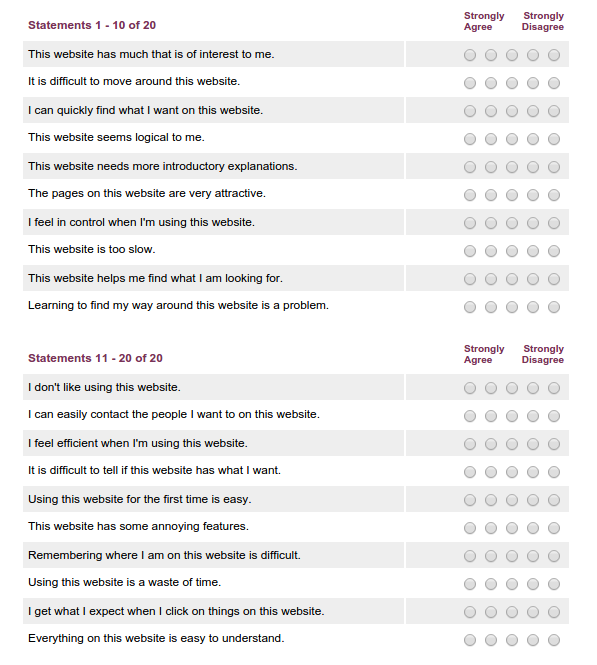
\includegraphics[scale=0.67]{editaveis/figuras/wammi_questions}
	\caption[Exemplo de itens do questionário WAMMI]{Exemplo de itens do questionário WAMMI. \footnotemark}
	\label{wammi_questions}
      \end{figure}
      
      As questões do WAMMI permitem analisar cinco fatores de usabilidade, Atratividade, Controlabilidade, Eficiência, Utilidade
      e Capacidade de aprendizado por meio de um padrão de resposta gradativo de cinco escalas que varia de “Concordo fortemente”
      a “Discordo fortemente”.
      \footnotetext{Disponível em: <http://www.wammi.com/samples/>.}
      
      Os serviços de análise das questões fornecidos pelo WAMMI são únicos, devido a todo arcabouço matemático e científico
      envolvido na sua construção, e, apesar do WAMMI ser voltado para \textit{websites}, para poder utilizá-lo no projeto, as perguntas
      podem ser adaptadas ao contexto do projeto para fornecer uma avaliação das metas de usabilidade Atratividade,
      Controlabilidade, Eficiência, Utilidade e Capacidade de aprendizado da aplicação.
    
    \subsection{\textit{Questionnaire for User Interface Satisfaction} - QUIS}
      
      \nocite{quis}
      O QUIS é um tipo de questionário que avalia a satisfação do usuário em relação a usabilidade do produto quanto à sua
      padronização, a fim de obter informações de forma precisa em relação a reação dos usuários aos seus novos produtos. 
      
      O pacote QUIS é composto por questões que podem ser avaliadas em uma escala de 0 a 9 e este pacote é possui um documento
      de texto composto por todas as seções do questionário que podem ser editadas de acordo com a necessidade de avaliação do 
      \textit{software}, possui uma versão única do questionário aplicado em HTML e possui também uma seleção dos trabalhos relevantes
      que detalham a validação do QUIS e alguns de seus usos. 
      
      O aplicativo \textit{MyPush} seguirá alguns padrões de interface para atender melhor a satisfação dos usuários na utilização do
      aplicativo. Esse tipo de questionário pode ser aplicado para garantir que a usabilidade seja levada em conta no processo de
      criação de interfaces do aplicativo e para verificar se o aplicativo está de conforme com as expectativas do usuário, 
      avaliando o seu grau de satisfação em relação as funcionalidades do \textit{MyPush}.
      
    \subsection{\textit{ErgoList}}
    
      O questionário ErgoList é um serviço disponibilizado via internet composto de uma base de conhecimento em ergonomia,
      que inspeciona, através de um \textit{checklist}, interfaces homem-computador. Nesse ambiente, o especialista avalia a interface 
      de uma aplicação usando o \textit{checklist} disponibilizado pelo LabIUtil. Tem uma base de questões bastante completa, cobrindo
      vários aspectos da usabilidade do \textit{software}. Por ser um \textit{checklist}, deve ser usado por um especialista com conhecimento em
      ergonomia (ERGOLIST, 2008).
      
      Este questionário leva em consideração os dezoito critérios ergonômicos de Bastien e Scapin (1993). São dezoito \textit{checklists}
      disponíveis no Ergolist, para cada um desses critérios que determina a ergonomia de uma interface homem-computador,
      totalizando 194 questões.
      
      O Ergolist é um questionário bem completo de tal modo que possui uma excelente precisão quando usado por um especialista,
      sendo muito útil para a medição.	

      Como o \textit{MyPush} é um aplicativo que pretende seguir os padrões de interface ditados pela indústria, é de vital
      importância para o seu desenvolvimento que estudos rígidos como o ErgoList sejam aplicados para que possa manter o 
      padrão desejado e o mesmo não fique aquém do esperado.
    
    \subsection{\textit{After Scenario Questionnaire} - ASQ}
    
      O questionário ASQ é um questionário feito para ser usado, como o próprio nome diz, imediatamente após cada cenário de uso
      completo, que permite avaliar a satisfação do usuário durante a participação de um estudo de usabilidade baseado em cenários,
      onde um cenário é um conjunto de tarefas relacionadas \cite{lewis91}.
      
      Consiste em apenas três itens que possuem padrão de resposta gradativo de sete escalas, que varia de “Concordo fortemente” 
      a “Discordo fortemente” e também conta com a opção “Não aplicável” fora da escala. A pontuação do questionário pode ser
      obtida pela média aritmética dos pontos de cada questão.
      
      \begin{figure}[h]
	\centering
	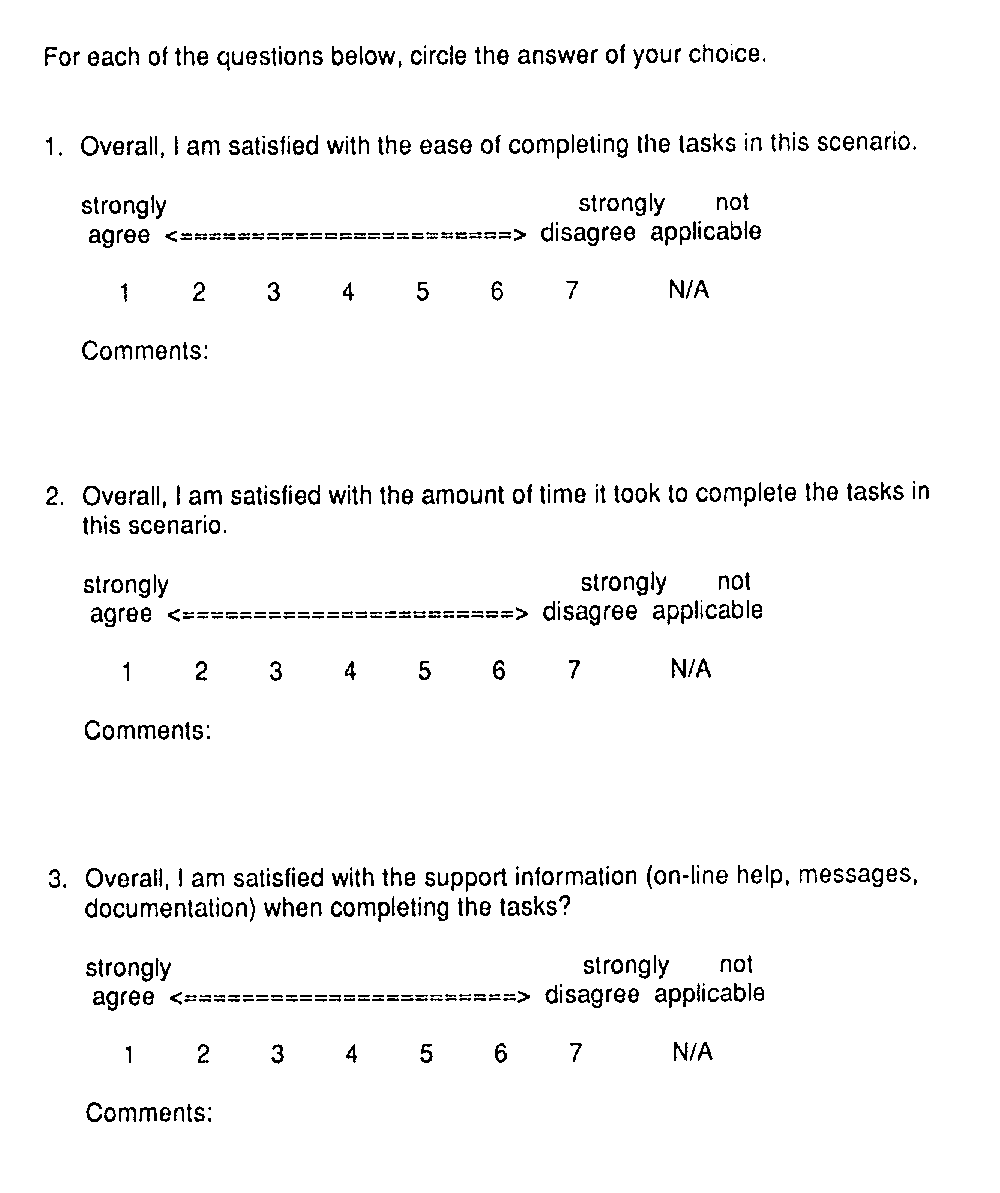
\includegraphics[scale=0.28]{editaveis/figuras/asq_questions}
	\caption[Questões do questionário ASQ]{Questões do questionário ASQ. Fonte: \cite{lewis91}.}
	\label{asq_questions}
      \end{figure}
      
      Os aspectos abordados nos itens do ASQ são: facilidade de completar as tarefas, tempo necessário para completar as tarefas 
      e satisfação com informações de suporte durante as tarefas, que possibilita visualizar a percepção do usuário a respeito da
      usabilidade do sistema \cite{lewis91}. A Figura ~\ref{asq_questions} mostra as três questões do ASQ.
      
      O questionário ASQ mostra se um recurso de avaliação rápido e eficaz para avaliar imediatamente a satisfação do usuário
      frente a um cenário de uso, evidenciando sua passividade de uso no projeto.
    
    \subsection{\textit{Post Study System Usability Questionnaire} - PSSUQ}
      
      O questionário PSSUQ é um instrumento que também permite avaliar a satisfação percebida pelo usuário ao utilizar um
      sistema \cite{lewis02}. Diferentemente do ASQ, o PSSUQ deve ser aplicado após completado um conjunto definido de cenários,
      para avaliar de forma generalizada o sistema (um conjunto de cenários).
      
      Assim como o ASQ, o PSSUQ também possui um padrão gradativo de resposta de sete escalas que varia de “Concordo fortemente”
      a “Discordo fortemente” e possui a opção “Não aplicável” fora da escala, porém conta com dezenove itens para a avaliação,
      onde cada item tem a possibilidade de receber um comentário do usuário. Os itens do PSSUQ (vide Figura ~\ref{pssuq_questions})
      permite avaliar o sistema em quatro dimensões, fornecendo medidas para cada um deles. São eles:
      
      \begin{itemize}
       \item \textit{SysUse} - Avalia a utilidade do sistema (\textit{System Usefulness}).
	  \subitem Questões 1-8;
      
       \item \textit{InfoQual} - Avalia a qualidade da informação fornecida pelo sistema. (\textit{Information Quality})
	  \subitem Questões 9-15;
	  
       \item \textit{InterQual} - Avalia a qualidade da interface do sistema (\textit{Interface Quality}).
	  \subitem Questões 16-18;
       
       \item \textit{Overall} - Avalia a satisfação geral do usuário com o sistema.
	  \subitem Questões 1-19.

      \end{itemize}
      
      Para obter a pontuação de qualquer área, basta calcular a média aritmética das pontuações das questões relacionadas à área.
      
      
      Um ponto interessante deste questionário é que, devido a utilização de técnicas psicométricas, a não observância de
      algumas questões não impacta significativamente no resultado obtido, ou seja, um questionário incompleto possui, 
      tecnicamente, a mesma confiabilidade de um questionário completo \cite{lewis02}. Outro ponto interessante é que o
      resultado do PSSUQ não possui variações significativas em detrimento ao sexo do usuário \cite{lewis02}.
      
      \vfill
      \pagebreak
      \begin{figure}[!htpb]
	\centering
	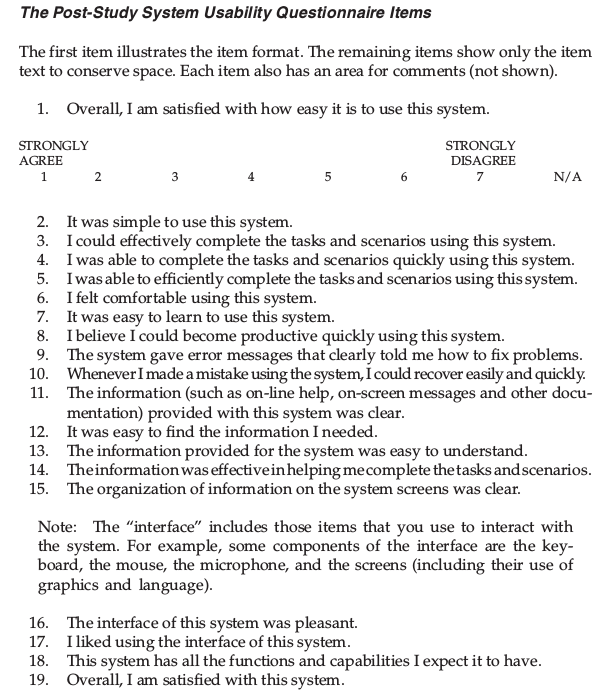
\includegraphics[scale=0.7]{editaveis/figuras/pssuq_questions}
	\caption[Questões do questionário PSSUQ]{Questões do questionário PSSUQ. Fonte: \cite{lewis02}.}
	\label{pssuq_questions}
      \end{figure}
      
      Com o que foi exposto, percebe-se que o PSSUQ é um questionário poderoso que permite uma avaliação confiável da
      satisfação do usuário em relação ao sistema. Como o PSSUQ deve ser utilizado após um conjunto de cenários ter sido
      completado, o seu uso concomitante com o ASQ se mostra uma prática promissora para a avaliação, pois, enquanto o ASQ
      retorna um feedback a cada cenário realizado, o PSSUQ permite um \textit{feedback} geral do sistema que está sendo analisado.
      
      \vfill
      
    \subsection{Questionários escolhidos}

      Foram escolhidos os questionários ASQ, para avaliação após cada cenário de uso, e PSSUQ, para a avaliação
      do conjunto de todos os cenários, que diz respeito ao produto final. 
      
      Os questionários escolhidos são satisfatórios para a realização
      da avaliação das metas definidas para a aplicação, pois ambos fornecem perguntas que permitem analisar tanto as metas 
      de usabilidade quanto as metas decorrentes da experiência do usuário estabelecidas, além de fornecerem um método numérico para 
      analisar os dados das entrevistas.
      